\documentclass[12pt, a4paper]{ctexart}
\usepackage{geometry}
\geometry{left=2.5cm, right=2.5cm, top=3cm, bottom=3cm}
\usepackage{graphicx}
\usepackage{xcolor}
\usepackage{circuitikz}
\usepackage{subcaption}
\usepackage{float}
\usepackage{amsmath}
\usepackage{listings}
\usetikzlibrary{arrows, shapes.gates.logic.US, positioning}
\ctikzset{
    logic ports=ieee,
    logic ports/scale=0.8,
    multipoles/flipflop/pin spacing=0.4
}
\lstset{
    basicstyle=\ttfamily\small,
    frame=single,
    framesep=5pt,
    xleftmargin=10pt,
    xrightmargin=10pt,
    keywordstyle=\color{blue},
    commentstyle=\color{gray},
    breaklines=true
}

\begin{document}

% 封面
\begin{titlepage}
    \centering
    \vspace*{5cm}
    {\Huge\bfseries 实验报告\par}
    \vspace{2cm}
    {\Large 课程：数字逻辑与计算机组成\par}
    \vspace{1cm}
    {\Large 实验四：运算部件设计\par}
    \vspace{4cm}
    {\large 姓名：\underline{\makebox[4cm]{郑袭明}}\par}
    \vspace{1cm}
    {\large 学号：\underline{\makebox[4cm]{251502027}}\par}
    \vspace{1cm}
    {\large 日期：\today\par}
\end{titlepage}

\tableofcontents
\enlargethispage{\baselineskip}
\newpage

\section{实验目的}

\begin{enumerate}
    \item 掌握先行进位部件 CLU 和先行进位加法器 CLA 的设计方法。
    \item 掌握 32 位快速加法器和标志位的设计方法。
    \item 掌握 32 位桶形移位器的设计方法。
    \item 掌握 RV32I 算术逻辑部件的设计方法。
\end{enumerate}

\section{实验一：4位先行进位加法器实验}

\subsection{整体方案设计}

首先设计特殊的全加器，有 $F=A\oplus B\oplus Cin,P=A+B,G=AB$

对于 CLU4，有

\begin{itemize}
    \item $C_1=G_0+P_0C_0$
    \item $C_2=G_1+P_1G_0+P_1P_0C_0$
    \item $C_3=G_2+P_2G_1+P_2P_1G_0+P_2P_1P_0C_0$
    \item $Pg=P_3P_2P_1P_0$
    \item $Gg=G_3+P_3G_2+P_3P_2G_1+P_3P_2P_1G_0$
    \item $C_4=Gg+PgC_0$
\end{itemize}

\begin{table}[H]
    \centering
    \begin{tabular}{|c|c|}
        \hline
        引脚 & 功能 \\
        \hline
        P[3:0] & 进位传递信号 \\
        G[3:0] & 进位产生信号 \\
        C[4:0] & 进位信号 \\
        Pg & 组进位传递信号 \\
        Gg & 组进位产生信号 \\
        \hline
    \end{tabular}
    \caption{4位先行进位部件引脚功能表}
\end{table}

拼接 CLU4 和 4 个特殊全加器即可得到 4 位先行进位加法器。

\begin{table}[H]
    \centering
    \begin{tabular}{|c|c|}
        \hline
        引脚 & 功能 \\
        \hline
        X[3:0] & 加数A \\
        Y[3:0] & 加数B \\
        Cin & 进位输入 \\
        Z[3:0] & 和 \\
        Cout & 进位输出 \\
        Pg & 组进位传递信号 \\
        Gg & 组进位产生信号 \\
        \hline
    \end{tabular}
    \caption{4位先行进位加法器引脚功能表}
\end{table}

\subsection{电路设计}

\begin{figure}[H]
    \centering
    
\includegraphics[width=0.8\textwidth]{assets/exp1/circuit1.png}
    \caption{4位先行进位加法器电路图}
\end{figure}

\begin{figure}[H]
    \centering
    
\includegraphics[width=0.8\textwidth]{assets/exp1/sch.png}
    \caption{4位先行进位部件原理图}
\end{figure}

\begin{figure}[H]
    \centering
    \subcaptionbox{4位先行进位部件}{
\includegraphics[width=0.55\textwidth]{assets/exp1/circuit2.png}}
    \subcaptionbox{特殊的全加器}{
\includegraphics[width=0.4\textwidth]{assets/exp1/circuit3.png}}
    \caption{4位先行进位部件电路图}
\end{figure}

\subsection{仿真结果}

\begin{figure}[H]
    \centering
    
\includegraphics[width=0.9\textwidth]{assets/exp1/sim1.png}
    \caption{4位先行进位加法器仿真结果(a)}
\end{figure}

\begin{figure}[H]
    \centering
    
\includegraphics[width=0.9\textwidth]{assets/exp1/sim2.png}
    \caption{4位先行进位加法器仿真结果(b)}
\end{figure}

\begin{table}[H]
    \centering
    \begin{tabular}{|c|c|c|c|}
        \hline
        Pg & Gg & Cin & Cout \\
        \hline
        X & 1 & X & 1 \\
        1 & 0 & 1 & 1 \\
        1 & 0 & 0 & 0 \\
        0 & 0 & X & 0 \\
        \hline
    \end{tabular}
    \caption{4位先行进位加法器真值表}
\end{table}

\subsection{错误现象及分析}

最开始看错了电路对应的表达式，导致连接错误；修改后连接正确。

\section{实验二：16位先行进位加法器实验}

\subsection{整体方案设计}

\begin{figure}[H]
    \centering
    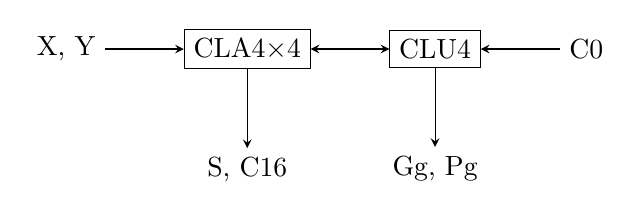
\begin{tikzpicture}[>=stealth]
        \node (XY) {X, Y};
        \node[draw, right=of XY] (CLA) {CLA4$\times$4};
        \node[draw, right=of CLA] (CLU) {CLU4};
        \node[below=of CLA] (S) {S, C16};
        \draw[->] (XY) -- (CLA);
        \draw[<->] (CLA) -- (CLU);
        \draw[->] (CLA) -- (S);
        \node[right=of CLU] (C0) {C0};
        \node[below=of CLU] (GgPg) {Gg, Pg};
        \draw[->] (C0) -- (CLU);
        \draw[->] (CLU) -- (GgPg);
    \end{tikzpicture}
    \caption{16位先行进位加法器整体方案设计}
\end{figure}

\begin{table}[H]
    \centering
    \begin{tabular}{|c|c|}
        \hline
        引脚 & 功能 \\
        \hline
        X[15:0] & 加数A \\
        Y[15:0] & 加数B \\
        C0 & 进位输入 \\
        S[15:0] & 和 \\
        C16 & 进位输出 \\
        Gg & 组进位产生信号 \\
        Pg & 组进位传递信号 \\
        \hline
    \end{tabular}
    \caption{16位先行进位加法器引脚功能表}
\end{table}

\subsection{电路设计}

\begin{figure}[H]
    \centering
    
\includegraphics[width=0.7\textwidth]{assets/exp2/sch.png}
    \caption{16位先行进位加法器原理图}
\end{figure}

\begin{figure}[H]
    \centering
    
\includegraphics[width=0.6\textwidth]{assets/exp2/circuit.png}
    \caption{16位先行进位加法器电路图}
\end{figure}

\subsection{仿真结果}

\begin{figure}[H]
    \centering
    \subcaptionbox{}{
\includegraphics[width=0.8\textwidth]{assets/exp2/sim1.png}}
    \subcaptionbox{}{
\includegraphics[width=0.8\textwidth]{assets/exp2/sim2.png}}
    \caption{16位先行进位加法器仿真结果}
\end{figure}

\begin{table}[H]
    \centering
    \begin{tabular}{|c|c|c|c|}
        \hline
        Pg & Gg & C0 & C16 \\
        \hline
        X & 1 & X & 1 \\
        1 & 0 & 1 & 1 \\
        1 & 0 & 0 & 0 \\
        0 & 0 & X & 0 \\
        \hline
    \end{tabular}
    \caption{16位先行进位加法器真值表}
\end{table}

\subsection{错误现象及分析}

在完成实验的过程中，没有遇到任何错误。

\section{实验三：32 位快速加法器实验}

\subsection{整体方案设计}

将两个16位先行进位加法器串联起来，前者的进位输出连接后者的进位输入，
同时前者的组进位产生信号和组进位传递信号连接后者的输入，
即可实现32位快速加法器。

\begin{table}[H]
    \centering
    \begin{tabular}{|c|c|}
        \hline
        引脚 & 功能 \\
        \hline
        X[31:0] & 加数A \\
        Y[31:0] & 加数B \\
        Cin & 进位输入 \\
        S[31:0] & 和 \\
        Cout & 进位输出 \\
        CF & 进位标志 \\
        OF & 溢出标志 \\
        SF & 符号标志 \\
        ZF & 零标志 \\
        \hline
    \end{tabular}
    \caption{32位快速加法器引脚功能表}
\end{table}

\subsection{电路设计}

\begin{figure}[H]
    \centering
    \subcaptionbox{原理图}{
\includegraphics[width=\textwidth]{assets/exp3/sch.png}}
    \subcaptionbox{电路图}{
\includegraphics[width=\textwidth]{assets/exp3/circuit.png}}
    \caption{32位快速加法器电路设计}
\end{figure}

\subsection{仿真结果}

\begin{figure}[H]
    \centering
    \subcaptionbox{}{
\includegraphics[width=0.8\textwidth]{assets/exp3/sim1.png}}
    \subcaptionbox{}{
\includegraphics[width=0.8\textwidth]{assets/exp3/sim2.png}}
        \caption{32位快速加法器仿真结果}
\end{figure}

\begin{table}[H]
    \centering
    \begin{tabular}{|c|c|}
        \hline
        引脚 & 输出 \\
        \hline
        CF & 当发生进位时为1，否则为0 \\
        OF & 当发生溢出时为1，否则为0 \\
        SF & 当结果为负数时为1，否则为0 \\
        ZF & 当结果为零时为1，否则为0 \\
        \hline
    \end{tabular}
    \caption{32位快速加法器真值表}
\end{table}

\subsection{错误现象及分析}

在完成实验的过程中，没有遇到任何错误。

\section{实验四：32位桶形移位器实验}

\subsection{整体方案设计}

\begin{lstlisting}[language=Verilog, caption={32位桶形移位器设计原理}]
module barrel (
    input [31:0] datain,
    input [4:0] shamt,
    input lr,
    input al,
    output reg [31:0] dataout
);

  always @(*) begin
    if (lr) dataout = datain << shamt;
    else if (al) dataout = ($signed(datain)) >>> shamt;
    else dataout = datain >> shamt;
  end

endmodule
\end{lstlisting}

\begin{table}[H]
    \centering
    \begin{tabular}{|c|c|}
        \hline
        引脚 & 功能 \\
        \hline
        datain[31:0] & 输入数据 \\
        shamt[4:0] & 移位量 \\
        lr & 左移/右移控制信号 \\
        al & 算术/逻辑控制信号 \\
        dataout[31:0] & 输出数据 \\
        \hline
    \end{tabular}
    \caption{32位桶形移位器引脚功能表}
\end{table}

\subsection{电路设计}

\begin{figure}[H]
    \centering
    \subcaptionbox{原理图}{
        \begin{circuitikz}
            \node[muxdemux,
                muxdemux def={Lh=6, Rh=6, NL=4, NB=0, NR=1},
            ] (shifter) at (0,0) {Shifter};
            \node[left] (datain) at (shifter.lpin 1) {datain[31:0]};
            \node[left] (shamt) at (shifter.lpin 2) {shamt[4:0]};
            \node[left] (lr) at (shifter.lpin 3) {lr};
            \node[left] (al) at (shifter.lpin 4) {al};
            \node[right] (dataout) at (shifter.rpin 1) {dataout[31:0]};
        \end{circuitikz}
    }
    \subcaptionbox{电路图}{
\includegraphics[width=\textwidth]{assets/exp4/circuit.png}}
    \caption{32位桶形移位器电路设计}
\end{figure}

\subsection{仿真结果}

\begin{figure}[H]
    \centering
    \subcaptionbox{}{
\includegraphics[width=0.8\textwidth]{assets/exp4/sim1.png}}
    \subcaptionbox{}{
\includegraphics[width=0.8\textwidth]{assets/exp4/sim2.png}}
    \subcaptionbox{}{
\includegraphics[width=0.8\textwidth]{assets/exp4/sim3.png}}
    \subcaptionbox{}{
\includegraphics[width=0.8\textwidth]{assets/exp4/sim4.png}}
    \caption{32位桶形移位器仿真结果}
\end{figure}

\begin{table}[H]
    \centering
    \begin{tabular}{|c|c|c|}
        \hline
        L/R & A/L & 输出 \\
        \hline
        0 & 0 & 逻辑右移 \\
        0 & 1 & 算术右移 \\
        1 & 0 & 逻辑左移 \\
        1 & 1 & 循环左移 \\
        \hline
    \end{tabular}
    \caption{32位桶形移位器真值表}
\end{table}

\subsection{错误现象及分析}

在完成实验的过程中，没有遇到任何错误。

\section{实验五：32位ALU实验}

\subsection{整体方案设计}

\begin{lstlisting}[language=Verilog, caption={}]
module alu (
    input [31:0] A,
    input [31:0] B,
    input [3:0] ALUctr,
    output zero,
    output reg [31:0] Result
);

  wire [4:0] shamt = B[4:0];
  wire less = (ALUctr[3] == 1'b0) ? ($signed(A) < $signed(B)) : (A < B);
  assign zero = (ALUctr[2:0] == 3'b010) ? (A == B) : (Result == 32'b0);

  always @(*) begin
    casez (ALUctr)
      4'b0000: Result = A + B;
      4'b1000: Result = A - B;
      4'b?001: Result = A << shamt;
      4'b?010: Result = {31'b0, less};
      4'b?011: Result = B;
      4'b?100: Result = A ^ B;
      4'b0101: Result = A >> shamt;
      4'b1101: Result = $signed(A) >>> shamt;
      4'b?110: Result = A | B;
      4'b?111: Result = A & B;
      default: Result = 32'b0;
    endcase
  end

endmodule
\end{lstlisting}

\begin{table}[H]
    \centering
    \begin{tabular}{|c|c|}
        \hline
        引脚 & 功能 \\
        \hline
        A[31:0] & 输入操作数A \\
        B[31:0] & 输入操作数B \\
        ALUctr[3:0] & ALU控制信号 \\
        zero & 零标志 \\
        Result[31:0] & ALU运算结果 \\
        \hline
    \end{tabular}
    \caption{32位ALU引脚功能表}
\end{table}

\subsection{电路设计}

\begin{figure}[H]
    \centering
    
\includegraphics[width=0.55\textwidth]{assets/exp5/circuit.png}
    \caption{32位ALU电路图}
\end{figure}

\begin{figure}[H]
    \centering
    
\includegraphics[width=0.75\textwidth]{assets/exp5/sch.png}
    \caption{32位ALU原理图}
\end{figure}

\subsection{仿真结果}

\begin{figure}[H]
    \centering
    \subcaptionbox{}{
\includegraphics[width=0.7\textwidth]{assets/exp5/sim1.png}}
    \subcaptionbox{}{
\includegraphics[width=0.7\textwidth]{assets/exp5/sim2.png}}
    \caption{32位ALU仿真结果(1)}
\end{figure}

\begin{figure}[H]
    \centering
    \subcaptionbox{}{
\includegraphics[width=0.7\textwidth]{assets/exp5/sim3.png}}
    \subcaptionbox{}{
\includegraphics[width=0.7\textwidth]{assets/exp5/sim4.png}}
    \caption{32位ALU仿真结果(2)}
\end{figure}

\begin{table}[H]
    \centering
    \begin{tabular}{|c|c|}
        \hline
        ALUctr & 运算 \\
        \hline
        0000 & 加法 \\
        1000 & 减法 \\
        ?001 & 逻辑左移 \\
        ?010 & 小于 \\
        ?011 & 直接输出B \\
        ?100 & 按位异或 \\
        0101 & 逻辑右移 \\
        1101 & 算术右移 \\
        ?110 & 按位或 \\
        ?111 & 按位与 \\
        \hline
    \end{tabular}
    \caption{32位ALU真值表}
\end{table}

\subsection{错误现象及分析}

在完成实验的过程中，没有遇到任何错误。

\end{document}
